\documentclass[twoside]{book}

% Packages required by doxygen
\usepackage{fixltx2e}
\usepackage{calc}
\usepackage{doxygen}
\usepackage[export]{adjustbox} % also loads graphicx
\usepackage{graphicx}
\usepackage[utf8]{inputenc}
\usepackage{makeidx}
\usepackage{multicol}
\usepackage{multirow}
\PassOptionsToPackage{warn}{textcomp}
\usepackage{textcomp}
\usepackage[nointegrals]{wasysym}
\usepackage[table]{xcolor}

% Font selection
\usepackage[T1]{fontenc}
\usepackage[scaled=.90]{helvet}
\usepackage{courier}
\usepackage{amssymb}
\usepackage{sectsty}
\renewcommand{\familydefault}{\sfdefault}
\allsectionsfont{%
  \fontseries{bc}\selectfont%
  \color{darkgray}%
}
\renewcommand{\DoxyLabelFont}{%
  \fontseries{bc}\selectfont%
  \color{darkgray}%
}
\newcommand{\+}{\discretionary{\mbox{\scriptsize$\hookleftarrow$}}{}{}}

% Page & text layout
\usepackage{geometry}
\geometry{%
  a4paper,%
  top=2.5cm,%
  bottom=2.5cm,%
  left=2.5cm,%
  right=2.5cm%
}
\tolerance=750
\hfuzz=15pt
\hbadness=750
\setlength{\emergencystretch}{15pt}
\setlength{\parindent}{0cm}
\setlength{\parskip}{3ex plus 2ex minus 2ex}
\makeatletter
\renewcommand{\paragraph}{%
  \@startsection{paragraph}{4}{0ex}{-1.0ex}{1.0ex}{%
    \normalfont\normalsize\bfseries\SS@parafont%
  }%
}
\renewcommand{\subparagraph}{%
  \@startsection{subparagraph}{5}{0ex}{-1.0ex}{1.0ex}{%
    \normalfont\normalsize\bfseries\SS@subparafont%
  }%
}
\makeatother

% Headers & footers
\usepackage{fancyhdr}
\pagestyle{fancyplain}
\fancyhead[LE]{\fancyplain{}{\bfseries\thepage}}
\fancyhead[CE]{\fancyplain{}{}}
\fancyhead[RE]{\fancyplain{}{\bfseries\leftmark}}
\fancyhead[LO]{\fancyplain{}{\bfseries\rightmark}}
\fancyhead[CO]{\fancyplain{}{}}
\fancyhead[RO]{\fancyplain{}{\bfseries\thepage}}
\fancyfoot[LE]{\fancyplain{}{}}
\fancyfoot[CE]{\fancyplain{}{}}
\fancyfoot[RE]{\fancyplain{}{\bfseries\scriptsize Generated by Doxygen }}
\fancyfoot[LO]{\fancyplain{}{\bfseries\scriptsize Generated by Doxygen }}
\fancyfoot[CO]{\fancyplain{}{}}
\fancyfoot[RO]{\fancyplain{}{}}
\renewcommand{\footrulewidth}{0.4pt}
\renewcommand{\chaptermark}[1]{%
  \markboth{#1}{}%
}
\renewcommand{\sectionmark}[1]{%
  \markright{\thesection\ #1}%
}

% Indices & bibliography
\usepackage{natbib}
\usepackage[titles]{tocloft}
\setcounter{tocdepth}{3}
\setcounter{secnumdepth}{5}
\makeindex

% Hyperlinks (required, but should be loaded last)
\usepackage{ifpdf}
\ifpdf
  \usepackage[pdftex,pagebackref=true]{hyperref}
\else
  \usepackage[ps2pdf,pagebackref=true]{hyperref}
\fi
\hypersetup{%
  colorlinks=true,%
  linkcolor=blue,%
  citecolor=blue,%
  unicode%
}

% Custom commands
\newcommand{\clearemptydoublepage}{%
  \newpage{\pagestyle{empty}\cleardoublepage}%
}

\usepackage{caption}
\captionsetup{labelsep=space,justification=centering,font={bf},singlelinecheck=off,skip=4pt,position=top}

%===== C O N T E N T S =====

\begin{document}

% Titlepage & ToC
\hypersetup{pageanchor=false,
             bookmarksnumbered=true,
             pdfencoding=unicode
            }
\pagenumbering{alph}
\begin{titlepage}
\vspace*{7cm}
\begin{center}%
{\Large Informatik Projekt }\\
\vspace*{1cm}
{\large Generated by Doxygen 1.8.14}\\
\end{center}
\end{titlepage}
\clearemptydoublepage
\pagenumbering{roman}
\tableofcontents
\clearemptydoublepage
\pagenumbering{arabic}
\hypersetup{pageanchor=true}

%--- Begin generated contents ---
\chapter{Namespace Index}
\section{Namespace List}
Here is a list of all namespaces with brief descriptions\+:\begin{DoxyCompactList}
\item\contentsline{section}{\mbox{\hyperlink{namespace_g_u_i_01_briefkasten}{G\+U\+I Briefkasten}} }{\pageref{namespace_g_u_i_01_briefkasten}}{}
\end{DoxyCompactList}

\chapter{Hierarchical Index}
\section{Class Hierarchy}
This inheritance list is sorted roughly, but not completely, alphabetically\+:\begin{DoxyCompactList}
\item object\begin{DoxyCompactList}
\item \contentsline{section}{Arduino}{\pageref{class_g_u_i_01_briefkasten_1_1_arduino}}{}
\item \contentsline{section}{Briefkasten\+Window}{\pageref{class_g_u_i_01_briefkasten_1_1_briefkasten_window}}{}
\item \contentsline{section}{Reset\+Button}{\pageref{class_g_u_i_01_briefkasten_1_1_reset_button}}{}
\end{DoxyCompactList}
\end{DoxyCompactList}

\chapter{Data Structure Index}
\section{Data Structures}
Here are the data structures with brief descriptions\+:\begin{DoxyCompactList}
\item\contentsline{section}{\mbox{\hyperlink{class_g_u_i_01_briefkasten_1_1_arduino}{Arduino}} }{\pageref{class_g_u_i_01_briefkasten_1_1_arduino}}{}
\item\contentsline{section}{\mbox{\hyperlink{class_g_u_i_01_briefkasten_1_1_briefkasten_window}{Briefkasten\+Window}} }{\pageref{class_g_u_i_01_briefkasten_1_1_briefkasten_window}}{}
\item\contentsline{section}{\mbox{\hyperlink{class_g_u_i_01_briefkasten_1_1_reset_button}{Reset\+Button}} }{\pageref{class_g_u_i_01_briefkasten_1_1_reset_button}}{}
\end{DoxyCompactList}

\chapter{File Index}
\section{File List}
Here is a list of all files with brief descriptions\+:\begin{DoxyCompactList}
\item\contentsline{section}{C\+:/\+Users/\+Adrian/\+Desktop/\+Liebe/\mbox{\hyperlink{_g_u_i_01_briefkasten_8py}{G\+U\+I Briefkasten.\+py}} }{\pageref{_g_u_i_01_briefkasten_8py}}{}
\end{DoxyCompactList}

\chapter{Namespace Documentation}
\hypertarget{namespace_g_u_i_01_briefkasten}{}\section{G\+UI Briefkasten Namespace Reference}
\label{namespace_g_u_i_01_briefkasten}\index{G\+U\+I Briefkasten@{G\+U\+I Briefkasten}}
\subsection*{Data Structures}
\begin{DoxyCompactItemize}
\item 
class \mbox{\hyperlink{class_g_u_i_01_briefkasten_1_1_arduino}{Arduino}}
\item 
class \mbox{\hyperlink{class_g_u_i_01_briefkasten_1_1_briefkasten_window}{Briefkasten\+Window}}
\item 
class \mbox{\hyperlink{class_g_u_i_01_briefkasten_1_1_reset_button}{Reset\+Button}}
\end{DoxyCompactItemize}
\subsection*{Variables}
\begin{DoxyCompactItemize}
\item 
\mbox{\hyperlink{namespace_g_u_i_01_briefkasten_a04a8a2bbfa9c15500892b8e5033d625b}{window}} = \mbox{\hyperlink{class_g_u_i_01_briefkasten_1_1_briefkasten_window}{Briefkasten\+Window}}()
\end{DoxyCompactItemize}


\subsection{Variable Documentation}
\mbox{\Hypertarget{namespace_g_u_i_01_briefkasten_a04a8a2bbfa9c15500892b8e5033d625b}\label{namespace_g_u_i_01_briefkasten_a04a8a2bbfa9c15500892b8e5033d625b}} 
\index{G\+U\+I Briefkasten@{G\+U\+I Briefkasten}!window@{window}}
\index{window@{window}!G\+U\+I Briefkasten@{G\+U\+I Briefkasten}}
\subsubsection{\texorpdfstring{window}{window}}
{\footnotesize\ttfamily window = \mbox{\hyperlink{class_g_u_i_01_briefkasten_1_1_briefkasten_window}{Briefkasten\+Window}}()}


\chapter{Data Structure Documentation}
\hypertarget{class_g_u_i_01_briefkasten_1_1_arduino}{}\section{Arduino Class Reference}
\label{class_g_u_i_01_briefkasten_1_1_arduino}\index{Arduino@{Arduino}}
Inheritance diagram for Arduino\+:\begin{figure}[H]
\begin{center}
\leavevmode
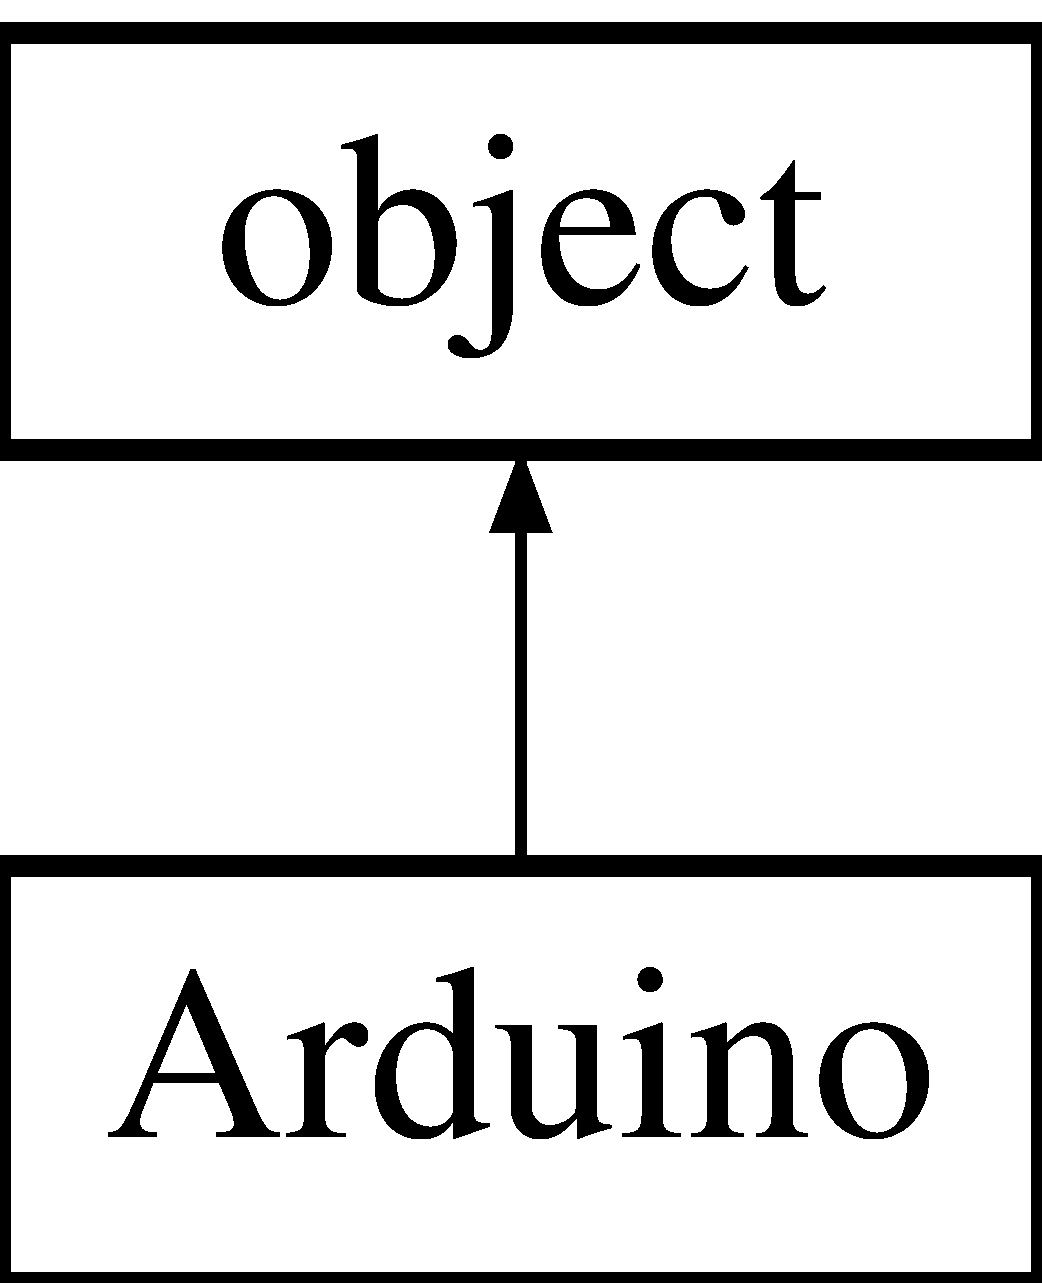
\includegraphics[height=2.000000cm]{class_g_u_i_01_briefkasten_1_1_arduino}
\end{center}
\end{figure}
\subsection*{Public Member Functions}
\begin{DoxyCompactItemize}
\item 
def \mbox{\hyperlink{class_g_u_i_01_briefkasten_1_1_arduino_a86404a4415caa006d76a1b7afa696fee}{\+\_\+\+\_\+init\+\_\+\+\_\+}} (self, \mbox{\hyperlink{class_g_u_i_01_briefkasten_1_1_arduino_a04a8a2bbfa9c15500892b8e5033d625b}{window}}, host, port, \mbox{\hyperlink{class_g_u_i_01_briefkasten_1_1_arduino_a7d39fd2404163714885928c07d431b76}{on\+\_\+received}})
\item 
def \mbox{\hyperlink{class_g_u_i_01_briefkasten_1_1_arduino_a05097bd2ea4ca3b2c17d7b7164a67539}{send\+\_\+command}} (self, command)
\item 
def \mbox{\hyperlink{class_g_u_i_01_briefkasten_1_1_arduino_a8639372c33e15084a7f7c4d9d87b7bfe}{close}} (self)
\end{DoxyCompactItemize}
\subsection*{Data Fields}
\begin{DoxyCompactItemize}
\item 
\mbox{\hyperlink{class_g_u_i_01_briefkasten_1_1_arduino_a04a8a2bbfa9c15500892b8e5033d625b}{window}}
\item 
\mbox{\hyperlink{class_g_u_i_01_briefkasten_1_1_arduino_a7d39fd2404163714885928c07d431b76}{on\+\_\+received}}
\item 
\mbox{\hyperlink{class_g_u_i_01_briefkasten_1_1_arduino_a84edc84c8145e7997b70f9919ce44d68}{socket}}
\item 
\mbox{\hyperlink{class_g_u_i_01_briefkasten_1_1_arduino_a1ea8c1aa4f00109a4c17150885fd08c8}{rd\+\_\+buff}}
\item 
\mbox{\hyperlink{class_g_u_i_01_briefkasten_1_1_arduino_a5299b01fe1537dddabd0e50400e0e9be}{after\+\_\+event}}
\end{DoxyCompactItemize}


\subsection{Constructor \& Destructor Documentation}
\mbox{\Hypertarget{class_g_u_i_01_briefkasten_1_1_arduino_a86404a4415caa006d76a1b7afa696fee}\label{class_g_u_i_01_briefkasten_1_1_arduino_a86404a4415caa006d76a1b7afa696fee}} 
\index{G\+U\+I Briefkasten\+::\+Arduino@{G\+U\+I Briefkasten\+::\+Arduino}!\+\_\+\+\_\+init\+\_\+\+\_\+@{\+\_\+\+\_\+init\+\_\+\+\_\+}}
\index{\+\_\+\+\_\+init\+\_\+\+\_\+@{\+\_\+\+\_\+init\+\_\+\+\_\+}!G\+U\+I Briefkasten\+::\+Arduino@{G\+U\+I Briefkasten\+::\+Arduino}}
\subsubsection{\texorpdfstring{\+\_\+\+\_\+init\+\_\+\+\_\+()}{\_\_init\_\_()}}
{\footnotesize\ttfamily def \+\_\+\+\_\+init\+\_\+\+\_\+ (\begin{DoxyParamCaption}\item[{}]{self,  }\item[{}]{window,  }\item[{}]{host,  }\item[{}]{port,  }\item[{}]{on\+\_\+received }\end{DoxyParamCaption})}



\subsection{Member Function Documentation}
\mbox{\Hypertarget{class_g_u_i_01_briefkasten_1_1_arduino_a8639372c33e15084a7f7c4d9d87b7bfe}\label{class_g_u_i_01_briefkasten_1_1_arduino_a8639372c33e15084a7f7c4d9d87b7bfe}} 
\index{G\+U\+I Briefkasten\+::\+Arduino@{G\+U\+I Briefkasten\+::\+Arduino}!close@{close}}
\index{close@{close}!G\+U\+I Briefkasten\+::\+Arduino@{G\+U\+I Briefkasten\+::\+Arduino}}
\subsubsection{\texorpdfstring{close()}{close()}}
{\footnotesize\ttfamily def close (\begin{DoxyParamCaption}\item[{}]{self }\end{DoxyParamCaption})}

\mbox{\Hypertarget{class_g_u_i_01_briefkasten_1_1_arduino_a05097bd2ea4ca3b2c17d7b7164a67539}\label{class_g_u_i_01_briefkasten_1_1_arduino_a05097bd2ea4ca3b2c17d7b7164a67539}} 
\index{G\+U\+I Briefkasten\+::\+Arduino@{G\+U\+I Briefkasten\+::\+Arduino}!send\+\_\+command@{send\+\_\+command}}
\index{send\+\_\+command@{send\+\_\+command}!G\+U\+I Briefkasten\+::\+Arduino@{G\+U\+I Briefkasten\+::\+Arduino}}
\subsubsection{\texorpdfstring{send\+\_\+command()}{send\_command()}}
{\footnotesize\ttfamily def send\+\_\+command (\begin{DoxyParamCaption}\item[{}]{self,  }\item[{}]{command }\end{DoxyParamCaption})}



\subsection{Field Documentation}
\mbox{\Hypertarget{class_g_u_i_01_briefkasten_1_1_arduino_a5299b01fe1537dddabd0e50400e0e9be}\label{class_g_u_i_01_briefkasten_1_1_arduino_a5299b01fe1537dddabd0e50400e0e9be}} 
\index{G\+U\+I Briefkasten\+::\+Arduino@{G\+U\+I Briefkasten\+::\+Arduino}!after\+\_\+event@{after\+\_\+event}}
\index{after\+\_\+event@{after\+\_\+event}!G\+U\+I Briefkasten\+::\+Arduino@{G\+U\+I Briefkasten\+::\+Arduino}}
\subsubsection{\texorpdfstring{after\+\_\+event}{after\_event}}
{\footnotesize\ttfamily after\+\_\+event}

\mbox{\Hypertarget{class_g_u_i_01_briefkasten_1_1_arduino_a7d39fd2404163714885928c07d431b76}\label{class_g_u_i_01_briefkasten_1_1_arduino_a7d39fd2404163714885928c07d431b76}} 
\index{G\+U\+I Briefkasten\+::\+Arduino@{G\+U\+I Briefkasten\+::\+Arduino}!on\+\_\+received@{on\+\_\+received}}
\index{on\+\_\+received@{on\+\_\+received}!G\+U\+I Briefkasten\+::\+Arduino@{G\+U\+I Briefkasten\+::\+Arduino}}
\subsubsection{\texorpdfstring{on\+\_\+received}{on\_received}}
{\footnotesize\ttfamily on\+\_\+received}

\mbox{\Hypertarget{class_g_u_i_01_briefkasten_1_1_arduino_a1ea8c1aa4f00109a4c17150885fd08c8}\label{class_g_u_i_01_briefkasten_1_1_arduino_a1ea8c1aa4f00109a4c17150885fd08c8}} 
\index{G\+U\+I Briefkasten\+::\+Arduino@{G\+U\+I Briefkasten\+::\+Arduino}!rd\+\_\+buff@{rd\+\_\+buff}}
\index{rd\+\_\+buff@{rd\+\_\+buff}!G\+U\+I Briefkasten\+::\+Arduino@{G\+U\+I Briefkasten\+::\+Arduino}}
\subsubsection{\texorpdfstring{rd\+\_\+buff}{rd\_buff}}
{\footnotesize\ttfamily rd\+\_\+buff}

\mbox{\Hypertarget{class_g_u_i_01_briefkasten_1_1_arduino_a84edc84c8145e7997b70f9919ce44d68}\label{class_g_u_i_01_briefkasten_1_1_arduino_a84edc84c8145e7997b70f9919ce44d68}} 
\index{G\+U\+I Briefkasten\+::\+Arduino@{G\+U\+I Briefkasten\+::\+Arduino}!socket@{socket}}
\index{socket@{socket}!G\+U\+I Briefkasten\+::\+Arduino@{G\+U\+I Briefkasten\+::\+Arduino}}
\subsubsection{\texorpdfstring{socket}{socket}}
{\footnotesize\ttfamily socket}

\mbox{\Hypertarget{class_g_u_i_01_briefkasten_1_1_arduino_a04a8a2bbfa9c15500892b8e5033d625b}\label{class_g_u_i_01_briefkasten_1_1_arduino_a04a8a2bbfa9c15500892b8e5033d625b}} 
\index{G\+U\+I Briefkasten\+::\+Arduino@{G\+U\+I Briefkasten\+::\+Arduino}!window@{window}}
\index{window@{window}!G\+U\+I Briefkasten\+::\+Arduino@{G\+U\+I Briefkasten\+::\+Arduino}}
\subsubsection{\texorpdfstring{window}{window}}
{\footnotesize\ttfamily window}



The documentation for this class was generated from the following file\+:\begin{DoxyCompactItemize}
\item 
C\+:/\+Users/\+Adrian/\+Desktop/\+Liebe/\mbox{\hyperlink{_g_u_i_01_briefkasten_8py}{G\+U\+I Briefkasten.\+py}}\end{DoxyCompactItemize}

\hypertarget{class_g_u_i_01_briefkasten_1_1_briefkasten_window}{}\section{Briefkasten\+Window Class Reference}
\label{class_g_u_i_01_briefkasten_1_1_briefkasten_window}\index{Briefkasten\+Window@{Briefkasten\+Window}}
Inheritance diagram for Briefkasten\+Window\+:\begin{figure}[H]
\begin{center}
\leavevmode
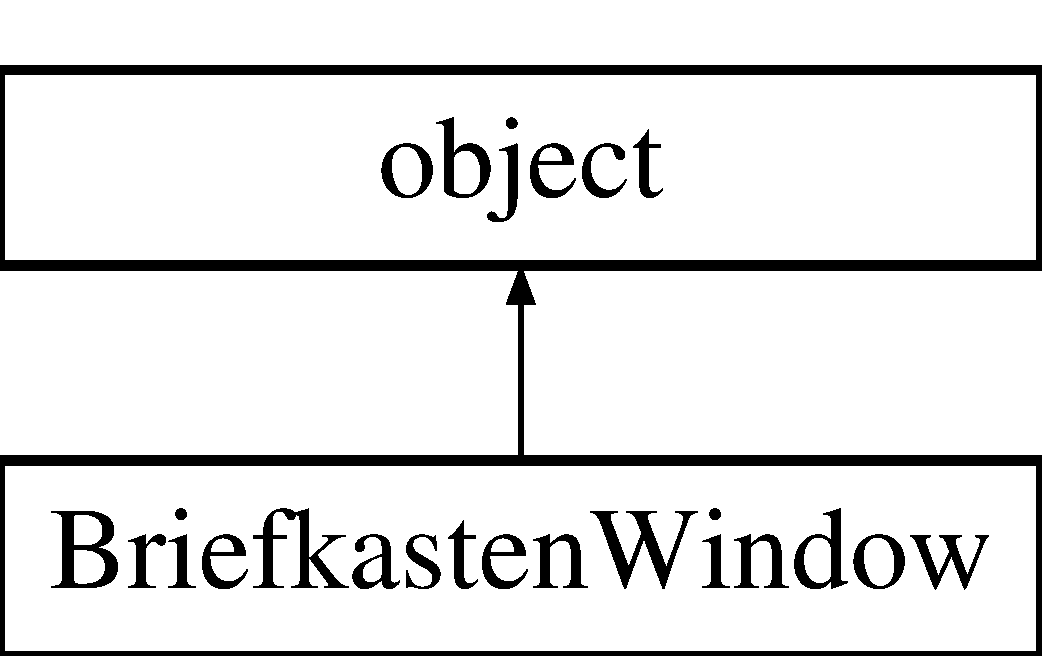
\includegraphics[height=2.000000cm]{class_g_u_i_01_briefkasten_1_1_briefkasten_window}
\end{center}
\end{figure}
\subsection*{Public Member Functions}
\begin{DoxyCompactItemize}
\item 
def \mbox{\hyperlink{class_g_u_i_01_briefkasten_1_1_briefkasten_window_ae64f0875afe3067b97ba370b354b9213}{\+\_\+\+\_\+init\+\_\+\+\_\+}} (self)
\item 
def \mbox{\hyperlink{class_g_u_i_01_briefkasten_1_1_briefkasten_window_ae427a00dd476d2fb2706445a342d9845}{on\+\_\+received}} (self, line)
\item 
def \mbox{\hyperlink{class_g_u_i_01_briefkasten_1_1_briefkasten_window_a9fe79fb8dbee1e660dc971b137c55f3f}{setup\+\_\+window}} (self)
\item 
def \mbox{\hyperlink{class_g_u_i_01_briefkasten_1_1_briefkasten_window_a7e20a417210b832ce9e307ce5dc0f2a8}{on\+\_\+close}} (self)
\item 
def \mbox{\hyperlink{class_g_u_i_01_briefkasten_1_1_briefkasten_window_ab6e6fe2e785e29f0597e4fcdd3ec9063}{setup\+\_\+content}} (self)
\item 
def \mbox{\hyperlink{class_g_u_i_01_briefkasten_1_1_briefkasten_window_ad22709b2e67308af35f55680d5a026e0}{run}} (self)
\end{DoxyCompactItemize}
\subsection*{Data Fields}
\begin{DoxyCompactItemize}
\item 
\mbox{\hyperlink{class_g_u_i_01_briefkasten_1_1_briefkasten_window_a3f424772edaa120b12bda2b9addc2bf5}{arduino}}
\item 
\mbox{\hyperlink{class_g_u_i_01_briefkasten_1_1_briefkasten_window_a04a8a2bbfa9c15500892b8e5033d625b}{window}}
\item 
\mbox{\hyperlink{class_g_u_i_01_briefkasten_1_1_briefkasten_window_a5db4d4152e9523bec44f0d385fb11e4c}{btn\+\_\+label\+\_\+var}}
\item 
\mbox{\hyperlink{class_g_u_i_01_briefkasten_1_1_briefkasten_window_a70069e35886a69852e6a41b1fb7a54be}{btn\+\_\+label}}
\item 
\mbox{\hyperlink{class_g_u_i_01_briefkasten_1_1_briefkasten_window_ab1f00069d86d1b1307d0b5e13a9765ae}{btn}}
\end{DoxyCompactItemize}


\subsection{Constructor \& Destructor Documentation}
\mbox{\Hypertarget{class_g_u_i_01_briefkasten_1_1_briefkasten_window_ae64f0875afe3067b97ba370b354b9213}\label{class_g_u_i_01_briefkasten_1_1_briefkasten_window_ae64f0875afe3067b97ba370b354b9213}} 
\index{G\+U\+I Briefkasten\+::\+Briefkasten\+Window@{G\+U\+I Briefkasten\+::\+Briefkasten\+Window}!\+\_\+\+\_\+init\+\_\+\+\_\+@{\+\_\+\+\_\+init\+\_\+\+\_\+}}
\index{\+\_\+\+\_\+init\+\_\+\+\_\+@{\+\_\+\+\_\+init\+\_\+\+\_\+}!G\+U\+I Briefkasten\+::\+Briefkasten\+Window@{G\+U\+I Briefkasten\+::\+Briefkasten\+Window}}
\subsubsection{\texorpdfstring{\+\_\+\+\_\+init\+\_\+\+\_\+()}{\_\_init\_\_()}}
{\footnotesize\ttfamily def \+\_\+\+\_\+init\+\_\+\+\_\+ (\begin{DoxyParamCaption}\item[{}]{self }\end{DoxyParamCaption})}



\subsection{Member Function Documentation}
\mbox{\Hypertarget{class_g_u_i_01_briefkasten_1_1_briefkasten_window_a7e20a417210b832ce9e307ce5dc0f2a8}\label{class_g_u_i_01_briefkasten_1_1_briefkasten_window_a7e20a417210b832ce9e307ce5dc0f2a8}} 
\index{G\+U\+I Briefkasten\+::\+Briefkasten\+Window@{G\+U\+I Briefkasten\+::\+Briefkasten\+Window}!on\+\_\+close@{on\+\_\+close}}
\index{on\+\_\+close@{on\+\_\+close}!G\+U\+I Briefkasten\+::\+Briefkasten\+Window@{G\+U\+I Briefkasten\+::\+Briefkasten\+Window}}
\subsubsection{\texorpdfstring{on\+\_\+close()}{on\_close()}}
{\footnotesize\ttfamily def on\+\_\+close (\begin{DoxyParamCaption}\item[{}]{self }\end{DoxyParamCaption})}

\mbox{\Hypertarget{class_g_u_i_01_briefkasten_1_1_briefkasten_window_ae427a00dd476d2fb2706445a342d9845}\label{class_g_u_i_01_briefkasten_1_1_briefkasten_window_ae427a00dd476d2fb2706445a342d9845}} 
\index{G\+U\+I Briefkasten\+::\+Briefkasten\+Window@{G\+U\+I Briefkasten\+::\+Briefkasten\+Window}!on\+\_\+received@{on\+\_\+received}}
\index{on\+\_\+received@{on\+\_\+received}!G\+U\+I Briefkasten\+::\+Briefkasten\+Window@{G\+U\+I Briefkasten\+::\+Briefkasten\+Window}}
\subsubsection{\texorpdfstring{on\+\_\+received()}{on\_received()}}
{\footnotesize\ttfamily def on\+\_\+received (\begin{DoxyParamCaption}\item[{}]{self,  }\item[{}]{line }\end{DoxyParamCaption})}

\mbox{\Hypertarget{class_g_u_i_01_briefkasten_1_1_briefkasten_window_ad22709b2e67308af35f55680d5a026e0}\label{class_g_u_i_01_briefkasten_1_1_briefkasten_window_ad22709b2e67308af35f55680d5a026e0}} 
\index{G\+U\+I Briefkasten\+::\+Briefkasten\+Window@{G\+U\+I Briefkasten\+::\+Briefkasten\+Window}!run@{run}}
\index{run@{run}!G\+U\+I Briefkasten\+::\+Briefkasten\+Window@{G\+U\+I Briefkasten\+::\+Briefkasten\+Window}}
\subsubsection{\texorpdfstring{run()}{run()}}
{\footnotesize\ttfamily def run (\begin{DoxyParamCaption}\item[{}]{self }\end{DoxyParamCaption})}

\mbox{\Hypertarget{class_g_u_i_01_briefkasten_1_1_briefkasten_window_ab6e6fe2e785e29f0597e4fcdd3ec9063}\label{class_g_u_i_01_briefkasten_1_1_briefkasten_window_ab6e6fe2e785e29f0597e4fcdd3ec9063}} 
\index{G\+U\+I Briefkasten\+::\+Briefkasten\+Window@{G\+U\+I Briefkasten\+::\+Briefkasten\+Window}!setup\+\_\+content@{setup\+\_\+content}}
\index{setup\+\_\+content@{setup\+\_\+content}!G\+U\+I Briefkasten\+::\+Briefkasten\+Window@{G\+U\+I Briefkasten\+::\+Briefkasten\+Window}}
\subsubsection{\texorpdfstring{setup\+\_\+content()}{setup\_content()}}
{\footnotesize\ttfamily def setup\+\_\+content (\begin{DoxyParamCaption}\item[{}]{self }\end{DoxyParamCaption})}

\mbox{\Hypertarget{class_g_u_i_01_briefkasten_1_1_briefkasten_window_a9fe79fb8dbee1e660dc971b137c55f3f}\label{class_g_u_i_01_briefkasten_1_1_briefkasten_window_a9fe79fb8dbee1e660dc971b137c55f3f}} 
\index{G\+U\+I Briefkasten\+::\+Briefkasten\+Window@{G\+U\+I Briefkasten\+::\+Briefkasten\+Window}!setup\+\_\+window@{setup\+\_\+window}}
\index{setup\+\_\+window@{setup\+\_\+window}!G\+U\+I Briefkasten\+::\+Briefkasten\+Window@{G\+U\+I Briefkasten\+::\+Briefkasten\+Window}}
\subsubsection{\texorpdfstring{setup\+\_\+window()}{setup\_window()}}
{\footnotesize\ttfamily def setup\+\_\+window (\begin{DoxyParamCaption}\item[{}]{self }\end{DoxyParamCaption})}



\subsection{Field Documentation}
\mbox{\Hypertarget{class_g_u_i_01_briefkasten_1_1_briefkasten_window_a3f424772edaa120b12bda2b9addc2bf5}\label{class_g_u_i_01_briefkasten_1_1_briefkasten_window_a3f424772edaa120b12bda2b9addc2bf5}} 
\index{G\+U\+I Briefkasten\+::\+Briefkasten\+Window@{G\+U\+I Briefkasten\+::\+Briefkasten\+Window}!arduino@{arduino}}
\index{arduino@{arduino}!G\+U\+I Briefkasten\+::\+Briefkasten\+Window@{G\+U\+I Briefkasten\+::\+Briefkasten\+Window}}
\subsubsection{\texorpdfstring{arduino}{arduino}}
{\footnotesize\ttfamily arduino}

\mbox{\Hypertarget{class_g_u_i_01_briefkasten_1_1_briefkasten_window_ab1f00069d86d1b1307d0b5e13a9765ae}\label{class_g_u_i_01_briefkasten_1_1_briefkasten_window_ab1f00069d86d1b1307d0b5e13a9765ae}} 
\index{G\+U\+I Briefkasten\+::\+Briefkasten\+Window@{G\+U\+I Briefkasten\+::\+Briefkasten\+Window}!btn@{btn}}
\index{btn@{btn}!G\+U\+I Briefkasten\+::\+Briefkasten\+Window@{G\+U\+I Briefkasten\+::\+Briefkasten\+Window}}
\subsubsection{\texorpdfstring{btn}{btn}}
{\footnotesize\ttfamily btn}

\mbox{\Hypertarget{class_g_u_i_01_briefkasten_1_1_briefkasten_window_a70069e35886a69852e6a41b1fb7a54be}\label{class_g_u_i_01_briefkasten_1_1_briefkasten_window_a70069e35886a69852e6a41b1fb7a54be}} 
\index{G\+U\+I Briefkasten\+::\+Briefkasten\+Window@{G\+U\+I Briefkasten\+::\+Briefkasten\+Window}!btn\+\_\+label@{btn\+\_\+label}}
\index{btn\+\_\+label@{btn\+\_\+label}!G\+U\+I Briefkasten\+::\+Briefkasten\+Window@{G\+U\+I Briefkasten\+::\+Briefkasten\+Window}}
\subsubsection{\texorpdfstring{btn\+\_\+label}{btn\_label}}
{\footnotesize\ttfamily btn\+\_\+label}

\mbox{\Hypertarget{class_g_u_i_01_briefkasten_1_1_briefkasten_window_a5db4d4152e9523bec44f0d385fb11e4c}\label{class_g_u_i_01_briefkasten_1_1_briefkasten_window_a5db4d4152e9523bec44f0d385fb11e4c}} 
\index{G\+U\+I Briefkasten\+::\+Briefkasten\+Window@{G\+U\+I Briefkasten\+::\+Briefkasten\+Window}!btn\+\_\+label\+\_\+var@{btn\+\_\+label\+\_\+var}}
\index{btn\+\_\+label\+\_\+var@{btn\+\_\+label\+\_\+var}!G\+U\+I Briefkasten\+::\+Briefkasten\+Window@{G\+U\+I Briefkasten\+::\+Briefkasten\+Window}}
\subsubsection{\texorpdfstring{btn\+\_\+label\+\_\+var}{btn\_label\_var}}
{\footnotesize\ttfamily btn\+\_\+label\+\_\+var}

\mbox{\Hypertarget{class_g_u_i_01_briefkasten_1_1_briefkasten_window_a04a8a2bbfa9c15500892b8e5033d625b}\label{class_g_u_i_01_briefkasten_1_1_briefkasten_window_a04a8a2bbfa9c15500892b8e5033d625b}} 
\index{G\+U\+I Briefkasten\+::\+Briefkasten\+Window@{G\+U\+I Briefkasten\+::\+Briefkasten\+Window}!window@{window}}
\index{window@{window}!G\+U\+I Briefkasten\+::\+Briefkasten\+Window@{G\+U\+I Briefkasten\+::\+Briefkasten\+Window}}
\subsubsection{\texorpdfstring{window}{window}}
{\footnotesize\ttfamily window}



The documentation for this class was generated from the following file\+:\begin{DoxyCompactItemize}
\item 
C\+:/\+Users/\+Adrian/\+Desktop/\+Liebe/\mbox{\hyperlink{_g_u_i_01_briefkasten_8py}{G\+U\+I Briefkasten.\+py}}\end{DoxyCompactItemize}

\hypertarget{class_g_u_i_01_briefkasten_1_1_reset_button}{}\section{Reset\+Button Class Reference}
\label{class_g_u_i_01_briefkasten_1_1_reset_button}\index{Reset\+Button@{Reset\+Button}}
Inheritance diagram for Reset\+Button\+:\begin{figure}[H]
\begin{center}
\leavevmode
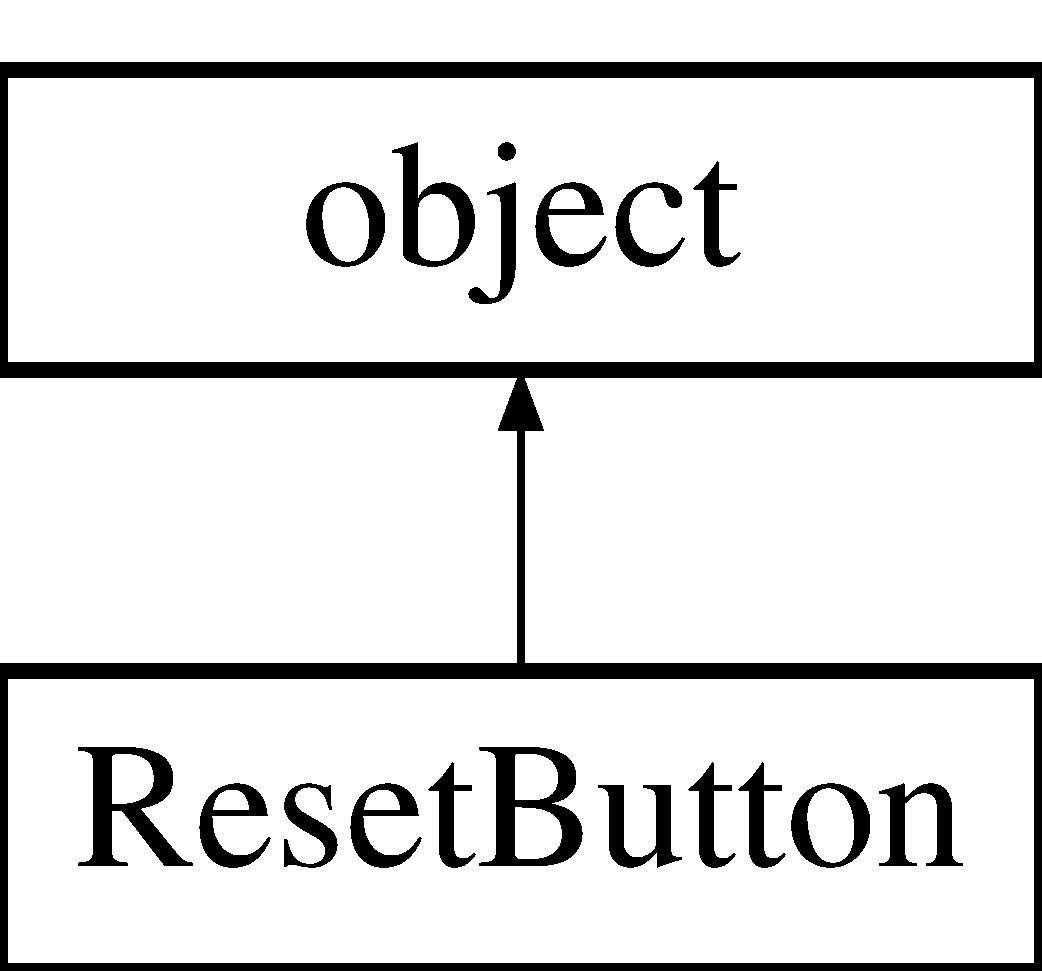
\includegraphics[height=2.000000cm]{class_g_u_i_01_briefkasten_1_1_reset_button}
\end{center}
\end{figure}
\subsection*{Public Member Functions}
\begin{DoxyCompactItemize}
\item 
def \mbox{\hyperlink{class_g_u_i_01_briefkasten_1_1_reset_button_a5f57538485260d20a41382d14a50b673}{\+\_\+\+\_\+init\+\_\+\+\_\+}} (self, \mbox{\hyperlink{namespace_g_u_i_01_briefkasten_a04a8a2bbfa9c15500892b8e5033d625b}{window}}, \mbox{\hyperlink{class_g_u_i_01_briefkasten_1_1_reset_button_a3f424772edaa120b12bda2b9addc2bf5}{arduino}})
\item 
def \mbox{\hyperlink{class_g_u_i_01_briefkasten_1_1_reset_button_ac59e8384988979b4ab58599ebe9dfe5e}{set\+\_\+state}} (self, \mbox{\hyperlink{class_g_u_i_01_briefkasten_1_1_reset_button_adc6e5733fc3c22f0a7b2914188c49c90}{state}})
\item 
def \mbox{\hyperlink{class_g_u_i_01_briefkasten_1_1_reset_button_a96da8e992148f9643251b6502b55e80f}{on\+\_\+pressed}} (self)
\end{DoxyCompactItemize}
\subsection*{Data Fields}
\begin{DoxyCompactItemize}
\item 
\mbox{\hyperlink{class_g_u_i_01_briefkasten_1_1_reset_button_a14139799dd4b2fc41ecb6cb14936322f}{button}}
\item 
\mbox{\hyperlink{class_g_u_i_01_briefkasten_1_1_reset_button_a3f424772edaa120b12bda2b9addc2bf5}{arduino}}
\item 
\mbox{\hyperlink{class_g_u_i_01_briefkasten_1_1_reset_button_adc6e5733fc3c22f0a7b2914188c49c90}{state}}
\end{DoxyCompactItemize}


\subsection{Detailed Description}
\begin{DoxyVerb}A button that controls one LED connected to an Arduino
while providing visual feedback of the current button state
\end{DoxyVerb}
 

\subsection{Constructor \& Destructor Documentation}
\mbox{\Hypertarget{class_g_u_i_01_briefkasten_1_1_reset_button_a5f57538485260d20a41382d14a50b673}\label{class_g_u_i_01_briefkasten_1_1_reset_button_a5f57538485260d20a41382d14a50b673}} 
\index{G\+U\+I Briefkasten\+::\+Reset\+Button@{G\+U\+I Briefkasten\+::\+Reset\+Button}!\+\_\+\+\_\+init\+\_\+\+\_\+@{\+\_\+\+\_\+init\+\_\+\+\_\+}}
\index{\+\_\+\+\_\+init\+\_\+\+\_\+@{\+\_\+\+\_\+init\+\_\+\+\_\+}!G\+U\+I Briefkasten\+::\+Reset\+Button@{G\+U\+I Briefkasten\+::\+Reset\+Button}}
\subsubsection{\texorpdfstring{\+\_\+\+\_\+init\+\_\+\+\_\+()}{\_\_init\_\_()}}
{\footnotesize\ttfamily def \+\_\+\+\_\+init\+\_\+\+\_\+ (\begin{DoxyParamCaption}\item[{}]{self,  }\item[{}]{window,  }\item[{}]{arduino }\end{DoxyParamCaption})}



\subsection{Member Function Documentation}
\mbox{\Hypertarget{class_g_u_i_01_briefkasten_1_1_reset_button_a96da8e992148f9643251b6502b55e80f}\label{class_g_u_i_01_briefkasten_1_1_reset_button_a96da8e992148f9643251b6502b55e80f}} 
\index{G\+U\+I Briefkasten\+::\+Reset\+Button@{G\+U\+I Briefkasten\+::\+Reset\+Button}!on\+\_\+pressed@{on\+\_\+pressed}}
\index{on\+\_\+pressed@{on\+\_\+pressed}!G\+U\+I Briefkasten\+::\+Reset\+Button@{G\+U\+I Briefkasten\+::\+Reset\+Button}}
\subsubsection{\texorpdfstring{on\+\_\+pressed()}{on\_pressed()}}
{\footnotesize\ttfamily def on\+\_\+pressed (\begin{DoxyParamCaption}\item[{}]{self }\end{DoxyParamCaption})}

\mbox{\Hypertarget{class_g_u_i_01_briefkasten_1_1_reset_button_ac59e8384988979b4ab58599ebe9dfe5e}\label{class_g_u_i_01_briefkasten_1_1_reset_button_ac59e8384988979b4ab58599ebe9dfe5e}} 
\index{G\+U\+I Briefkasten\+::\+Reset\+Button@{G\+U\+I Briefkasten\+::\+Reset\+Button}!set\+\_\+state@{set\+\_\+state}}
\index{set\+\_\+state@{set\+\_\+state}!G\+U\+I Briefkasten\+::\+Reset\+Button@{G\+U\+I Briefkasten\+::\+Reset\+Button}}
\subsubsection{\texorpdfstring{set\+\_\+state()}{set\_state()}}
{\footnotesize\ttfamily def set\+\_\+state (\begin{DoxyParamCaption}\item[{}]{self,  }\item[{}]{state }\end{DoxyParamCaption})}



\subsection{Field Documentation}
\mbox{\Hypertarget{class_g_u_i_01_briefkasten_1_1_reset_button_a3f424772edaa120b12bda2b9addc2bf5}\label{class_g_u_i_01_briefkasten_1_1_reset_button_a3f424772edaa120b12bda2b9addc2bf5}} 
\index{G\+U\+I Briefkasten\+::\+Reset\+Button@{G\+U\+I Briefkasten\+::\+Reset\+Button}!arduino@{arduino}}
\index{arduino@{arduino}!G\+U\+I Briefkasten\+::\+Reset\+Button@{G\+U\+I Briefkasten\+::\+Reset\+Button}}
\subsubsection{\texorpdfstring{arduino}{arduino}}
{\footnotesize\ttfamily arduino}

\mbox{\Hypertarget{class_g_u_i_01_briefkasten_1_1_reset_button_a14139799dd4b2fc41ecb6cb14936322f}\label{class_g_u_i_01_briefkasten_1_1_reset_button_a14139799dd4b2fc41ecb6cb14936322f}} 
\index{G\+U\+I Briefkasten\+::\+Reset\+Button@{G\+U\+I Briefkasten\+::\+Reset\+Button}!button@{button}}
\index{button@{button}!G\+U\+I Briefkasten\+::\+Reset\+Button@{G\+U\+I Briefkasten\+::\+Reset\+Button}}
\subsubsection{\texorpdfstring{button}{button}}
{\footnotesize\ttfamily button}

\mbox{\Hypertarget{class_g_u_i_01_briefkasten_1_1_reset_button_adc6e5733fc3c22f0a7b2914188c49c90}\label{class_g_u_i_01_briefkasten_1_1_reset_button_adc6e5733fc3c22f0a7b2914188c49c90}} 
\index{G\+U\+I Briefkasten\+::\+Reset\+Button@{G\+U\+I Briefkasten\+::\+Reset\+Button}!state@{state}}
\index{state@{state}!G\+U\+I Briefkasten\+::\+Reset\+Button@{G\+U\+I Briefkasten\+::\+Reset\+Button}}
\subsubsection{\texorpdfstring{state}{state}}
{\footnotesize\ttfamily state}



The documentation for this class was generated from the following file\+:\begin{DoxyCompactItemize}
\item 
C\+:/\+Users/\+Adrian/\+Desktop/\+Liebe/\mbox{\hyperlink{_g_u_i_01_briefkasten_8py}{G\+U\+I Briefkasten.\+py}}\end{DoxyCompactItemize}

\chapter{File Documentation}
\hypertarget{_g_u_i_01_briefkasten_8py}{}\section{C\+:/\+Users/\+Adrian/\+Desktop/\+Liebe/\+G\+UI Briefkasten.\+py File Reference}
\label{_g_u_i_01_briefkasten_8py}\index{C\+:/\+Users/\+Adrian/\+Desktop/\+Liebe/\+G\+U\+I Briefkasten.\+py@{C\+:/\+Users/\+Adrian/\+Desktop/\+Liebe/\+G\+U\+I Briefkasten.\+py}}
\subsection*{Data Structures}
\begin{DoxyCompactItemize}
\item 
class \mbox{\hyperlink{class_g_u_i_01_briefkasten_1_1_arduino}{Arduino}}
\item 
class \mbox{\hyperlink{class_g_u_i_01_briefkasten_1_1_reset_button}{Reset\+Button}}
\item 
class \mbox{\hyperlink{class_g_u_i_01_briefkasten_1_1_briefkasten_window}{Briefkasten\+Window}}
\end{DoxyCompactItemize}
\subsection*{Namespaces}
\begin{DoxyCompactItemize}
\item 
 \mbox{\hyperlink{namespace_g_u_i_01_briefkasten}{G\+U\+I Briefkasten}}
\end{DoxyCompactItemize}
\subsection*{Variables}
\begin{DoxyCompactItemize}
\item 
\mbox{\hyperlink{namespace_g_u_i_01_briefkasten_a04a8a2bbfa9c15500892b8e5033d625b}{window}} = Briefkasten\+Window()
\end{DoxyCompactItemize}

%--- End generated contents ---

% Index
\backmatter
\newpage
\phantomsection
\clearemptydoublepage
\addcontentsline{toc}{chapter}{Index}
\printindex

\end{document}
